\chapter{Related work}
\label{chap:related_work}
In this chapter, the most relevant studies on the classification of music-elicited emotions have been reviewed. In 2013 T. Eerola and J. Vuoskoski \cite{eerola_review_2013} reviewed and categorized 251 studies related to music and emotions in terms of approaches, emotion models and stimuli. However, most of them are not comparable in terms of methods with the current study and the list is not updated with the most recent findings in the field of \ac{ER}. Therefore, the selection of studies reported below features some very well-known foundational ones that provide the theoretical framework to approach the selection of relevant features and the analysis of emotions using physiological signals, and some more recent ones focused on the classification of music-elicited emotions using machine learning algorithms. They have been ordered chronologically to emphasize the methodological progresses and their contribution to the design of the current experimental protocol and classification methods has been highlighted where appropriate. However, to underline the novelty of this research, only one reviewed study features the use of a wearable \ac{EEG} headset with 8 dry electrodes and another one artificially simulates the use of wearable device by picking 2 frontal electrodes from a bigger dataset recorded with 32 wet electrodes.

\section{Classification of music-elicited emotions}
\label{sec:classification_emotions}
L.A. Schmidt and L.J. Trainor \cite{schmidt_frontal_2001} were the first investigators that reviewed all the existing regional brain activation/emotion models and tried to systematically verify their validity for the analysis of music-elicited emotions. To do so, they designed an experiment selecting 4 orchestral excerpts that were pre-rated to represent the following classes:
\begin{enumerate}
\item Intense-unpleasant emotion: fear
\item Intense-pleasant emotion: joy
\item Calm-pleasant emotion: happy
\item Calm-unpleasant emotion: sad
\end{enumerate}
They hypothesized that:

\begin{itemize}
\item “Asymmetric frontal activation reflects emotional valence”
\begin{itemize}
\item Greater relative left frontal EEG activity for joy and happy musical pieces
\item Greater relative right frontal EEG activity for fear and sad musical pieces
\end{itemize}
\item “Regional brain activation reflects emotional intensity”
\begin{itemize}
\item A significant main effect for the intensity of affective musical excerpts on overall frontal \ac{EEG} activity is characterized by a frontal pattern that would distinguish across valence as predicted by Davidson, Schmidt, and Dawson.
\item Right parietal activity would distinguish the intensity of the affective musical excerpts across valence as predicted by Heller.
\end{itemize}
\end{itemize}
Then, they recruited 59 participants (30 females) right-handed undergraduates of psychology between 18 and 34. Their EEG signal was recorded continuously for 60 seconds for each musical excerpt. The data was pre-processed and cleaned from artefacts, then analysed using \ac{DFT} with a Hanning window of 1-second width and 50\% overlap. 

\begin{figure}[h!]
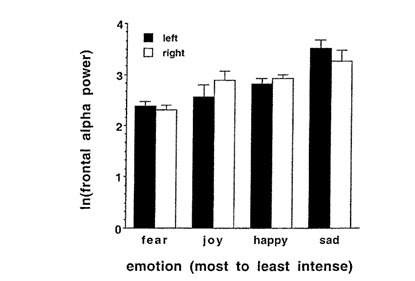
\includegraphics[width=10cm]{img/related_work/valence_hemisphere.png}
\centering
\caption{Valence by hemisphere interaction showed differences among the four musical excerpts on the left and right frontal EEG alpha power. Taken from \cite{schmidt_frontal_2001}}\label{fig_schmidt_valence_emo}
\end{figure}
Frequency-band specific power in the alpha band (8-13Hz) was derived from the \ac{DFT} output over the complete power spectrum. ANOVA analysis on Valence by Hemisphere interaction revealed a consistent behaviour between the left frontal EEG activity with positive valence songs and between the right frontal \ac{EEG} activity with negative valence songs (Fig. \ref{fig_schmidt_valence_emo}).
According to their findings, they could confirm that asymmetrical frontal activation indeed distinguished the valence of musical emotion: subjects exhibited greater relative left frontal EEG activity for musical excerpts with positive valence and vice versa on the right side for musical excerpts with negative valence (Fig. \ref{fig_schmidt_valence_alpha}), confirming their first hypothesis. Furthermore, the results showed that musically induced emotions elicit the same frontal brain regions as emotions induced through other means, which validates musical stimuli as good emotional elicitors for agnostic emotion classification. Intensity by hemisphere analysis reported main effects on intensity, but without interaction: subjects showed significantly greater activity in the frontal region as the affective stimuli became more intense. 

\begin{figure}[h!]
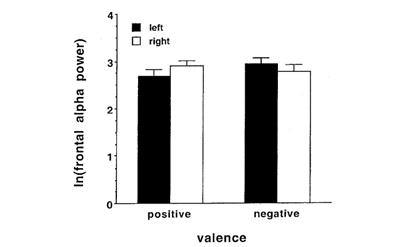
\includegraphics[width=10cm]{img/related_work/valence_hemisphere_alpha.png}
\centering
\caption{Valence by hemisphere interaction.Alpha power is inversely related to activity, positive left is accordingly lower for positive emotions and negative right is lower for negative emotion. Taken from \cite{schmidt_frontal_2001}}\label{fig_schmidt_valence_alpha}
\end{figure}
The frontal \ac{EEG} activity decreased from the presentation of the fear to the joy to the happy to the sad excerpts and it is consistent with the behavioural rating of intensity. Since they only used auditory stimuli, the lack of parietal differences might be due to the lack of external focus from environmental stimuli. 

\begin{figure}[h!]
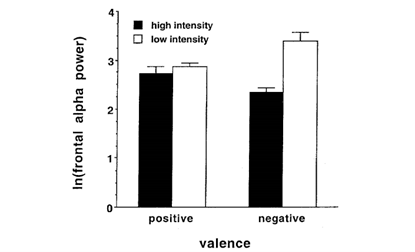
\includegraphics[width=10cm]{img/related_work/valence_intensity.png}
\centering
\caption{Valence by intensity interaction. Greater power (lower activity) in the low-intensity excerpts than in higher intensity excerpts, with a more extreme difference for negative valenced excerpts. Taken from \cite{schmidt_frontal_2001}}\label{fig_schmidt_valence_intensity}
\end{figure}
Valence by Intensity analysis showed that musical excerpts with higher intensity and positive valence elicited significantly higher activity compared with the opposite combination, low intensity and negative valence (Fig. \ref{fig_schmidt_valence_intensity}). This study is relevant for the analysis of music-elicited emotions because it provides a validation for the models proposed by Davidson, Fox and Heller that state the approach-withdrawal tendencies in the frontal \ac{EEG} activity: positive emotions are processed in the left anterior region of the brain, negative emotions are processed in the right anterior region of the brain. Regarding the intensity, or arousal dimension, of the emotions, the results are consistent with the models by Davidson, Dawson and Schmidt that correlate absolute frontal activation with the intensity of the emotional experience. However, in contrast with Heller’s model, they did not find relevant differences in the right parietal activity, possibly because of their experimental setup.
\\
\\
In 2009, Lin et al. \cite{lin_eeg-based_2009} recorded 26 participants to perform Emotion-Recognition of four emotional states representing the 4 quadrants of the \ac{VA} space: joy, pleasure, sadness, and anger. They proposed the listening of pre-labelled emotional music and then collected the discrete self-reported labels from their subjects to be used for classification. After removing motion artifacts with visual inspection, they extracted the frequency-band specific power in the theta, alpha, beta and gamma bands using\ac{STFT} and then derived the power of each \ac{EEG} component across time over 32-channels. They calculated 12 asymmetry indexes (ASM12) as the difference in power from 12 symmetric electrode pairs for at total 60 features over five \ac{EEG} components. \ac{SVM} was used to classify the data in three different configurations:
•	“all-together”: multi-class in one step with Crammer’s optimization formulation
•	“one-against-one”:  binary classification for K(K-1)/2 classifiers, then the test prediction is decided with max wins strategy.
•	“model-based”: two-level nested binary classifiers, one for valence and one for arousal, then the results are aggregated.
The they then proceeded with a subject-dependent strategy for classification. They obtained the best performance with the “one-against-one” scheme, respectively 94.86 \% (1.76) accuracy for valence and 94.43\% (2.12) for arousal and showed that the binary classification strategy is consistently more reliable than multi-class classification. However, there are no reports about the distribution of the self-reported labels, meaning we do not know if the datasets were balanced or unbalanced between the four emotional states.
\\
\\
In 2010, a remarkable comparison of modern methods can be found in a subsequent study from Y. Lin et al. \cite{lin_eeg-based_2010}, which developed a systematic framework for optimization of EEG-based emotion recognition. According to the asymmetry and regional activation theories, they extracted a set of spectral features (PSD30) from Delta, Theta, Alpha, Beta and Gamma frequency-band specific power. Subsequently, they derived several asymmetry indexes by power subtraction (DASM12) or division (RASM12) between 12 symmetrical pairs of 24 electrodes placed over the frontal, central and parietal areas of the brain and lastly, they also used the individual spectra of these 24 electrodes (PSD24). They then proceeded with automatic feature selection to improve the accuracy of the classification of four emotional states, namely joy, anger, sadness, and pleasure, testing subject-dependent classification with both \ac{SVM} and \ac{MLP}. After F-score ranking all the features by performance, they identified which features were subject-independent to the whole dataset. Finally, they repeated the experiment lowering the number of electrodes and features, and they compared the performance of both subject-independent and subject-dependent features.

\begin{figure}[h!]
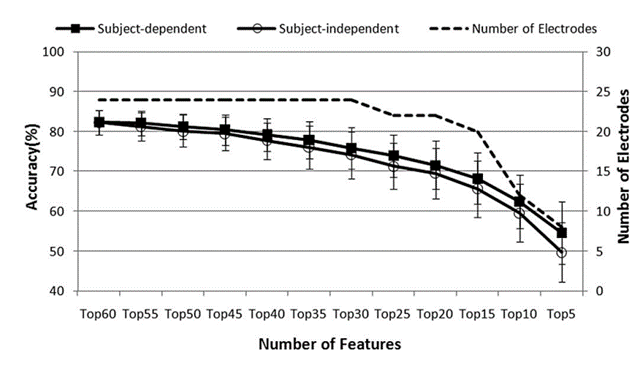
\includegraphics[width=12cm]{img/related_work/lin_features_ranking.png}
\centering
\caption{Comparison of average accuracy of subject-dependent and independent features and the number of electrodes for subject-independent features. Taken from \cite{lin_eeg-based_2010}}\label{fig_lin_features_ranking}
\end{figure}

According to the classification results, differential asymmetry features (DASM12) yielded better accuracy than rational asymmetry features (RASM12), Furthermore, DASM12 significantly improved classification performances compared to PSD24, even if they were derived from the same electrodes, suggesting that hemispheric power asymmetry is more discriminating in the measurement of mental states. These differential asymmetries were also subject-independent, meaning that their performance was consistent across subjects. In addition, further experiments on electrodes reduction proved the classification performance to be quite comparable despite the lower number of features, and only dramatically declined when the number of features was reduced below 10 (see Fig. \ref{fig_lin_features_ranking}). This study provides useful insights on the performances of features based on hemispheric asymmetry. However, it is hard to compare with other works or the current study, because of the decision to report classification performances of 4 emotional classes created from the aggregated dimensions in the valence-arousal space.
\\
\\
In 2013, Koelstra et al. \cite{koelstra_deap_2012} created one of the biggest public available datasets, both in terms of participants and variety of signals collected, to investigate the emotion recognition task using physiological signals. They investigated the role of emotions in communication and realized that most systems fail in interpreting the human emotional vocabulary, they are not able to identify emotional states and use them accordingly. According to the authors, the goal of affective computing is to fill this gap and synthesize emotional responses. Affective characteristics are features that can describe multimedia content and can be associated with implicit emotional tags. These tags could then be used to improve the performance of recommendation and retrieval systems in understanding the user’s taste and then recommend content that matches the current emotion.
They adopted a three-dimensional model that adds third dimension to Russel’s valence-arousal model: dominance. Arousal ranges from inactive to active, valence ranges from unpleasant to pleasant and finally dominance ranges from a “helpless and weak” feeling to an “empowered” feeling. They utilized \ac{SAM} \cite{bradley_measuring_1994} for the self-reporting task of discrete emotions.
Physiological signals seem to carry emotional information; they comprise signals from the \ac{CNS} and \ac{PNS} as well (see Fig. \ref{fig_koelstra_sensors}). They are available to be used for emotion assessment but were not in the main scope of the experiment. Music videos were used as visual stimuli, 32 participants (16 females) took part in the experiment and their \ac{EEG} and peripheral physiological signals were recorded while they were watching 40 selected stimuli. They were asked to rate each video in terms of arousal, valence, like/dislike, dominance, and familiarity and for 22 of them the frontal face video was also recorded.
After several steps of semi-automatic selection of 120 stimuli and a manual selection for the rest, 40 final stimuli were selected, considering an equal distribution between the 4 quadrants/classes that can be identified in the valence-arousal space:
\begin{itemize}
\item 	\textbf{LALV} : low arousal / low valence
\item 	\textbf{LAHV}: low arousal / high valence
\item  	\textbf{HALV}: high arousal / low valence
\item     \textbf{HAHV}: high arousal / high valence
\end{itemize}


For each selected music video, they extracted a 1-minute segment and used an affective highlighting algorithm by Soleymani et al \cite{soleymani_bayesian_2009}. Between each segment, there were 55 seconds of overlap, content features were extracted and provided the input for the regressors. The emotional highlight score was computed with the following equation: 
\[ e_i= \sqrt{a_i^2 + v_i^2} \]
Where \emph{a} is the arousal, \emph{v} is the valence and \(e_i\) is the i-th  segment of emotional highlight. For each video, the segment with the highest score was extracted for the experiment.

\begin{figure}[h!]
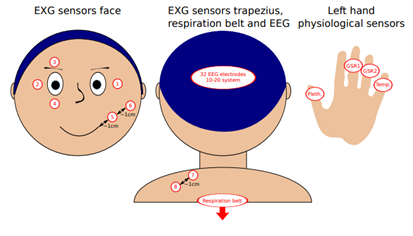
\includegraphics[width=12cm]{img/related_work/koelstra_sensors.png}
\centering
\caption{Placement of physiological sensors to record EOG, EMG, GSR, BVP, temperature and respiration. Taken from \cite{koelstra_deap_2012}.}\label{fig_koelstra_sensors}
\end{figure}

The experiment included 2 minutes recording of the baseline, then the 40 videos were presented in 40 trials, each consisting of:
\begin{itemize}
\item 2-second screen displaying the current trial number
\item 5-second baseline recording
\item 1-minute display of the music video
\item Self-assessment for arousal, valence, liking and dominance
\end{itemize}
The stimuli from the four conditions, in general, elicited the target emotion (see Fig. 12) and high-arousing conditions worked particularly well.

\begin{figure}[h!]
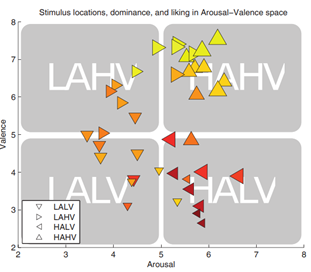
\includegraphics[width=8cm]{img/related_work/koelstra_va_space.png}
\centering
\caption{ Mean location of the stimuli on the Valence-Arousal space for the 4 classes. Liking is colour-coded as red for low and bright yellow for high, while dominance is size-coded with small symbols for low and big symbols for high.Taken from \cite{koelstra_deap_2012}.}\label{fig_koelstra_va_space}
\end{figure}

Emotions with strong valence and low arousal were instead more difficult to elicit. They also observed a high positive correlation between liking and valence, and between dominance and valence, meaning that people liked music that gave them a positive feeling or feeling of empowerment. Medium positive correlations were observed between arousal and dominance and between arousal and liking. Familiarity correlated with liking and valence moderately and positively.
They found negative correlations for arousal in the Theta, Alpha and Gamma band, with the central Alpha power decreasing for higher arousal, that matched the findings of their previous study. There is also an inverse relationship between alpha power and the general level of arousal. Valence instead showed the strongest correlation with \ac{EEG} signals in all the frequency bands. In Theta and Alpha frequency bands, an increase in valence led to an increase in power. For the Beta frequency, there are a central decrease and an occipital and right temporal increase of power, associated with positive emotional self-induction and external stimulation. Liking correlates could be found in all frequency bands, for Theta and Alpha power they showed an increase over the left frontocentral cortices. In summary, their observed correlations partially concur with their previous study and other studies that explore the neurophysiological correlates of affective states. 

\begin{figure}[h!]
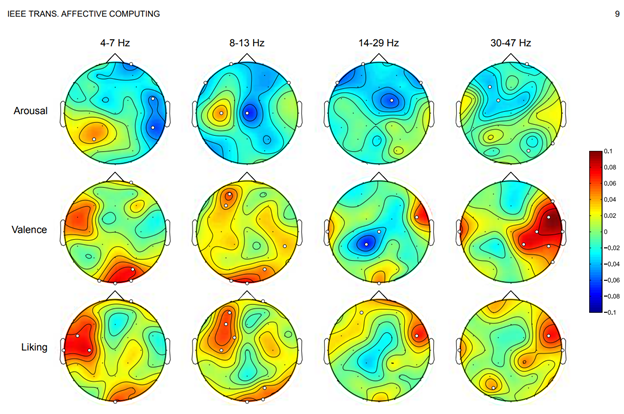
\includegraphics[width=12cm]{img/related_work/koelstra_topomaps.png}
\centering
\caption{Mean correlations overall participants of valence, arousal, and rating with power in Theta, Alpha, Beta and Gamma bands. Highlighted sensors are significantly correlated with the ratings.Taken from \cite{koelstra_deap_2012}.}\label{fig_koelstra_topomaps}
\end{figure}

To preprocess the \ac{EEG} data, the signal was down sampled, high pass filtered using EEGLab and then eye artifacts were removed with blind source separation technique using the recorded \ac{EOG}. Classification was experimented in three modalities: \ac{EEG} signals, peripheral physiological signals, and \ac{MCA}, but only the first one is relevant for the current study. Power spectral features were extracted from the \ac{EEG} signal in the theta, alpha, beta, and gamma bands, then the asymmetry was measured as difference in spectral power from symmetrical pairs of electrodes. In total they used 216 \ac{EEG} features for single trial subject-dependent classification with leave-one-out cross validation scheme, where one stimulus was used as test set at each step of the cross validation. Many datasets where unbalanced in the distribution of valence and arousal labels, thus used F1-score to assess the reliability of the accuracy scores. Using a gaussian naïve Bayesian classifier, they reported an average accuracy of 62\% for arousal classification with F1-score of 0.583, and an average accuracy of 57.6\% for valence classification with F1-score of 0.563. The results were compared against random guessing, class ration and default majority class guessing. The F1-score distribution was significantly higher than 0.5, indicating the models’ capability to learn from \ac{EEG} features despite unbalanced datasets and average accuracy lower than majority class guessing.
\\
\\
Reuderik, Mühl and Poel \cite{reuderink_valence_2013} investigated correlations between emotional valence, arousal, and dominance during game play to study affective correlates in a realistic and uncontrolled environment. To induce frustration, they utilized a game designed to ignore 15\% of keyboard input for short periods, with the screen lagging to simulate an under-powered computer. They recruited 12 healthy users and asked them to play the game through a sequence of random permutations of two normal games and one frustrating game of 2 minutes each. After each game, the subjects were asked to self-report their current mental state using Self-Assessment Manikins. During the experimental session, they were recorded with a BioSemi ActiveTwo EEG system with 32 active electrodes placed at the extended locations of the 10-20 system. In addition, \ac{EOG} were recorded to measure the influence of ocular artifacts and \ac{EMG} to record the finger movement used to control the game. The \ac{EEG} data were high pass filtered to remove frequencies below 0.2Hz and notch filtered to remove power line noise, then the signal was corrected for eye movements using linear regression analysis subtraction. Finally, the data was re-referenced to the \ac{CAR}. For the feature extraction, they estimated the power in different frequencies using Welch’s method for each experimental game session, then within each session they summed the log-power in the Alpha band for each electrode and subtracted the band power of electrodes on the left hemisphere from the corresponding electrodes on the right hemisphere. The obtained Alpha-asymmetry indexes for each sensor pair were used to find a correlate with valence. The results of the statistical correlations of self-reported valence, arousal and dominance confirmed correlates for both valence and arousal in the Theta, Delta, and Alpha frequency-band specific powers during the activity of gaming. The different affective dimension did not seem to be orthogonal, valence and dominance ratings were highly correlated, thus effects found in the \ac{EEG} related to one affective dimension can be attributed to the other. Their conclusions on frequency-specific and localized emotional interpretation are valuable for the current study, despite the use of a video-game as elicitor. The asymmetry of Alpha power and fronto-central Theta power were validated for the measurement of emotional valence. Right frontal Alpha power and the absence of right parietal Delta power instead were instead indicative of the arousal dimension. They conclude stating that these effects and the stronger narrow-band effects could be used for automatic recognition of affect. The importance of this study lies in the validation of the asymmetry and regional absolute activation theories in a realistic scenario, which is of fundamental importance in the pursuit of real-time \ac{ER}.
\\
\\
The data-oriented approach in the study from Thammasan et al.  \cite{thammasan_continuous_2016}  in 2016 focused on considering emotional oscillations within a single music piece during EEG-based emotion recognition. They proposed a continuous emotion-recognition approach, including self-reporting and continuous emotion annotation using the VA model. After adopting two different approaches for information extraction, \ac{FD} and \ac{PSD}, they discovered that \ac{FD} slightly outperforms \ac{PSD} in both arousal and valence subject-dependent classification, while having a higher correlation between the classification and self-reported emotions. \ac{FD} is an alternative approach to the analysis of irregular time series, proposed by T. Higuchi \cite{higuchi_approach_1988}, and is now getting more popularity in affective computing research, because of a relative simplicity compared to \ac{PSD}. Higher values of FD reflect the higher activity of the brain; \ac{PSD} instead indicates the signal power in specific frequency ranges, and it’s based on fast Fourier transform, used to decompose the EEG signal into the previously explained frequency ranges: delta, theta, alpha, beta, and gamma. EEG-based emotion recognition is promising for potential applications like music therapy, multimedia tagging, and multimedia retrieval. However, previous studies did not consider emotion variation and usually adopted a single emotion annotation approach because the experiments were run with music excerpts shorter than a minute. Since emotions are subjective and the same piece of music can induce different emotions in listeners, they also gathered self-annotated emotion labels from them. This can overcome the problem that many studies have, i.e. the use of pre-emotion-labelled music pieces from standard libraries, where emotions are labelled by an expert or by other users. For the experimental session, they recorded 15 male participants between 22 and 30, all healthy students from Osaka University. The music collection was composed of 40 pieces in MIDI format, so that additional emotions contributed by lyrics could be eliminated. The 12 electrodes used were chosen for their location close to the frontal lobe, the part of the brain that is crucial for emotion regulation: Fp1, Fp2, F3, F4, F7, F8, Fz, C3, C4, T3, T4, and Pz. Each song length was on average two minutes, then followed by 16 seconds of silent rests to allow the participant to mitigate the effects from the previous song when starting the next one. After the listening session, the participants listened to the same songs and annotated their perceived emotions by clicking on the corresponding points in the valence arousal emotion space. For feature extraction, they applied a sliding window segmentation that could analyse temporal data to track emotional fluctuation. A window of 1000 samples was used, equivalent to 4 seconds. To perform emotion classification, emotional tagging in one window was set to a high or positive value if the number of positive instances was greater than the number of negative instances. Using feature extraction with the two approaches, they obtained 12 features from \ac{FD} value calculation and 60 features with \ac{PSD}. Since traditional methodologies neglected emotional changes over time, they decided to compare the continuous recognition with the traditional method by simulating it with a sliding window size expanded to the full length of the song. The “chance level” was introduced for annotated emotion to provide a benchmark to evaluate models since annotated data could be unevenly distributed in terms of positive/negative perception. In this way, the chance level is defined by the majority class of the training data (with 60\% positive samples, the chance level would be 60\%).

\begin{figure}[h!]
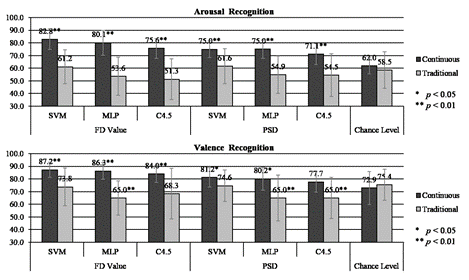
\includegraphics[width=12cm]{img/related_work/thammasan_cont_results.png}
\centering
\caption{Average classification accuracy and standard deviation for valence and arousal across all subjects .Taken from \cite{thammasan_continuous_2016}.}\label{fig_thammasan_cont_results}
\end{figure}

The results (see Fig. \ref{fig_thammasan_cont_results}) show that all the continuous approaches, regardless of the algorithm used, outperform the traditional method. Classification with \ac{FD} features using \ac{SVM} achieved the best relative result of 82.8\% for arousal recognition with a chance level of 62\%. Also in valence recognition, \ac{FD} features proved to perform better with \ac{SVM} and the highest accuracy of 87.2\%. The general higher arousal correlation of \ac{FD} value features might be the reason it performed better than \ac{PSD} for arousal recognition, and similarly, they could achieve better results for valence recognition because of their slightly higher absolute correlations. The results obtained with \ac{PSD} features are later compared with the results obtained in the current study, that also used features extracted from \ac{PSD} (see Chapter \ref{sec:comparison}).
\\
\\
Wu et al. \cite{wu_estimation_2017}  experimented valence classification on the DEAP dataset \cite{koelstra_deap_2012} in 2017 using a small subset of channels located in the frontal area selected according to the asymmetry theory, to simulate the use of a wearable device.
They extracted spectral properties using \ac{FFT})and calculated the following features:
\begin{itemize}
\item 	Entropy to measure the randomness of a signal in the Delta and Gamma frequency bands.
\item 	\ac{SASI} to detect emotions based on a balance between power in Theta and Beta frequency bands as defined in Chapter 2.7.
\item 	\ac{EVI} that reflects the hemisphere asymmetry of frontal Theta power similarly to \ac{AWI} and  calculated as: \[EVI=\frac{10(\log_{10}(TF\theta PL) - \log_{10}(TF\theta PR)}{(\log_{10}(TF\theta PL) + \log_{10}(TF\theta PR)}\]
\end{itemize}
They also calculated differential asymmetry indexes based on the power in Beta (BASI), Delta (DASI) and Gamma (GASI) frequency bands, for a total of 68 features for classification. After building a multi-classifier system for subject-dependent classification, they obtained the best performance with a \ac{GBDT} classifier that scored a maximum valence classification accuracy of 76.34\% and a mean accuracy of 75.15\% using only two frontal electrodes, Fp1 and Fp2. They repeated the experiment with 4 and 6 frontal electrodes as shown in Figure 15 only slightly improving the performance.  The subject-independent experiment with leave-one-subject-out scored sensibly worse, with an average accuracy of 61.82\%, having highest accuracy of 91.67\% and lowest accuracy of 21.43\%. Furthermore, to consider the unbalance towards the positive valence class, the authors labelled each trial as positive if the valence score was higher than 7 and negative if the valence score was lower than 3, but it is not clear how the trial is labelled for a value in between nor what is the actual distribution of labels for each subject.

\begin{figure}[h!]
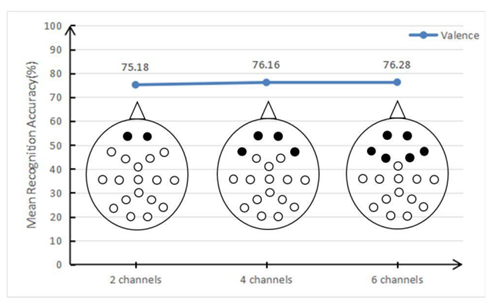
\includegraphics[width=12cm]{img/related_work/wu_electrodes.png}
\centering
\caption{Mean classification accuracy with 3 different subsets of electrodes from DEAP. Taken from  \cite{wu_estimation_2017}.}\label{fig_wu_electrodes}
\end{figure}


These results proves that classification is possible with a meagre amount of electrodes, but also that strategically selected frontal electrodes contain enough affective information to eventually perform the classification task using a wearable device and with a lower computational cost, thus more suitable for real-time classification. However, subject-independent classification seems to be highly affected by subject-dependent variations, thus less promising. The authors also did not mention their preprocessing strategy, and this fact is only explainable if they used the already preprocessed version of the DEAP dataset, made available by the authors in the same package with the raw data. This study is valuable for the investigation of Emotion-Recognition with a simulated wearable device but does not give further insights for a realistic real-time application.
\\
\\
Also in 2017, Thammasan et al. \cite{thammasan_multimodal_2017} presented a framework for adaptive multi-modal recognition using a dataset collected recording the \ac{EEG}, \ac{ECG} and \ac{GSR} signals of 9 healthy subjects listening to music. This study is the only one based on a wearable \ac{EEG} headset with 8 soft dry electrodes developed by IMEC. All the musical stimuli were selected based on previous studies and with statistically verified emotional ratings, simplified to 4 classes corresponding to the quadrants of the \ac{VA} space. They also utilized a stratified music-selection approach, with a selection of 16 songs from the researchers themselves, and 8 songs subject-selected. They then proceeded with the experiment, collecting the \ac{VA} labels with continuous annotation using the mouse and SAM \cite{bradley_measuring_1994} in a scale from 1 to 9 after each trial, followed by a rating of familiarity in a scale from 1 to 5 to verify the overall familiarity with the music. They also collected whether the subjects liked or not the song and their confidence in the self-rated annotations on a scale from 1 to 3. The PREP \cite{bigdely-shamlo_prep_2015} preprocessing pipeline was run in EEGLAB with standard filtering and \ac{ICA} decomposition to remove eye movement activity and muscular artifacts. The \ac{EEG} features were extracted using multi-taper \ac{PSD} to minimizing bias and more robust under stochasticity. \ac{PSD} features were extracted in the theta, alpha, beta and gamma frequency bands, but no further differential or rational computation was applied. Classification was performed with \ac{SVM} based on RBF kernel with subject-dependent strategy. For each subject, emotional valence and arousal were classified with leave-one-block-out cross-validation, then\ac{MCC} scores were calculated to give a more accurate representation of the classification performances with unbalanced classes. This is one of the first reviewed studies to clearly consider the unbalance of classes that is typical of emotion related studies involving music, and the accuracy performances are compare against the “chance level” of each subject, which is defined as majority-voting accuracy. The performances of the classification are evaluated as multi-modal contribution of several physiological sources, but the maximum accuracy obtained by \ac{EEG} as uni-modal source is ~80\% for valence and ~72\% for arousal. Unfortunately, no detailed accuracy scores are provided, but instead the \ac{MCC} scores are presented for each modality. The average \ac{MCC} score for valence is 0.247 (0.17) with the highest score being 0.596 (0.3), while the average \ac{MCC} score for arousal is 0.177 (0.04) and the highest score being 0.23 (0.22). Given the impact of personal perception on the distribution of emotional labels, \ac{MCC} is an important evaluation metric as later explained, when discussing the optimization process of the current research (see Chapter \ref{sec:optimizations}).
\\
\\
Recently, Keelawal et al.\cite{keelawat_comparative_2021} followed up their study \cite{thammasan_continuous_2016}, comparing the use of the deep learning algorithm \ac{CNN}, with other methods for emotion recognition on \ac{EEG} signals. \ac{CNN} has shown very good results and potential in the generalization of unseen subjects, therefore they aimed to study how to tune the hyper-parameters to obtain beneficial optimizations. Their results show that the temporal information in distinct window sizes significantly affects the recognition performance, and \ac{CNN} was more responsive to window changes than \ac{SVM}. Subject-independent classification with (\ac{LOSO} strategy and 10-fold cross-validation of arousal achieved highest accuracy of 56.85\% and \ac{MCC} of 0.1369, window size of 10 seconds, while valence recognition performed a highest accuracy of 73.34\% and \ac{MCC} of 0.4669 with an 8 second window size. \ac{CNN} has been recently applied to EEG-based emotion recognition with the advantage of circumventing feature engineering and improving classification accuracy thanks to its advantages at capturing adjacent spatial information. The fact that emotional responses can evolve creates the necessity of continuous annotation of emotions to allow capturing the temporal dynamic of emotion. Spatial information is also important using \ac{CNN} the placement of adjacent electrodes in the input matrix can be impactful, meaning the accuracy can be improved with an optimal arrangement of the order of \ac{EEG} electrodes over the most contributing regions of the brain in emotional processing.
The experiment was conducted with 12 male students from Osaka University, using a collection of 40 MIDI files, which were equally distributed over the four quadrants of the arousal-valence space. Subjects were instructed to select 8 familiar songs and 8 unfamiliar songs. Each song was played for 2 minutes with a 16 second silence interval in between. The electrodes were chosen near the frontal lobe. After listening to the songs, the subjects were detached from the \ac{EEG} equipment and were asked to listen again in the same order and annotate the emotions by clicking on the arousal-valence space at the corresponding position (every 2-3 seconds). During the \ac{EEG} pre-processing a band-pass filter was applied (0.5-60Hz) and \ac{ICA} was computed using the Info-Max algorithm and then the components were evaluated based on the power spectral density, scalp topography, and location of the equivalent current dipole.
Four different architectures were tested with respectively 3, 4, 5 and 6 convolutional layers and the same model as represented in Figure \ref{fig_keelawal_architecture}. 

\begin{figure}[h!]
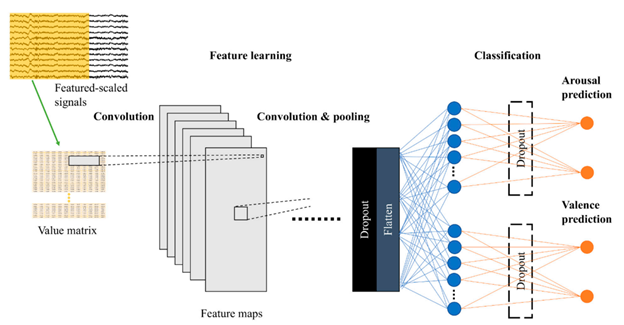
\includegraphics[width=12cm]{img/related_work/keelawal_architecture.png}
\centering
\caption{Optimized architecture of the model in  \cite{keelawat_comparative_2021}.}\label{fig_keelawal_architecture}
\end{figure}

Increasing the window frame led to higher performance in all \ac{CNN} architectures, for both arousal and valence, with a higher improvement of the valence condition considering the \ac{MCC} ranges of both conditions (0.1302 for valence and 0.0951 for arousal). Arousal classification scored the best results with window size of 10 seconds, obtaining 56.85\% accuracy and \ac{MCC} value of 0.1369, and scored the lowest with a 1-second window size obtaining 52.09\% accuracy and \ac{MCC} of 0.0418. On the other hand, valence classification obtained the best accuracy at 73.34\% with a window size of 8 seconds and \ac{MCC} value of 0.4669, while the lowest accuracy was 66.83\% and \ac{MCC} of 0.3367 with 1-second window size. According to these results, there could be enormous variations between the signal of each subject and expanding the window size could reduce fluctuations among distinct subjects. Compared to their previous work using \ac{SVM} (linear, polynomial and RBF kernels) on the same EEG dataset, the window size was way more influential for \ac{CNN}. Electrode sorting instead had less marked effects on the classification in comparison with a random order, with 3D Physical order for valence classification obtaining significant differences with 72.94\% accuracy and \ac{MCC} of 0.4588. MinCBO also had some significant improvement overall. The results of subject-independent classification in this experiment seems to confirm that strategy is achievable with computationally demanding offline pre-processing pipelines and a fine-tuning process of the deep learning models. These considerations, together with the use of a standard \ac{EEG} headset, suggest that subject-independent classification might be still too challenging for real-time Emotion-Recognition using a wearable device. 
\\
\\
The general trend of investigating Emotion-Recognition using \ac{EEG} is to support the task with discrete or continuous emotion annotations to reduce the biasing effects of pre-labelled emotional labels, as well as selecting the recording channels that are positionally more relevant in the analysis of emotional processing in the brain. Fractal Dimension algorithms and Power Spectral Density calculation seem to be the most promising pre-processing techniques for feature extraction. The reviewed studies focus on the frontal asymmetrical hemispheric tendencies in the alpha and theta powers, which are usually computed as differential or rational indexes between symmetrical pair of electrodes. The absolute activation in frequency-band specific Theta, Alpha, Beta and Gamma powers in the frontal, central and parietal area are all relevant in the study of emotions, but there was not a prominent method for features computation. The limitation of the \ac{EEG} equipment used for the current study, as well as the light preprocessing approach, constrained the analysis so that only frontal Theta, Alpha and Beta frequency-band specific powers were considered. Machine learning algorithms, like Linear Regression, \ac{GBDT} and \ac{SVM}, but also deep learning algorithms like \ac{MLP} and \ac{CNN}, were possible valid choices for the task, depending on the amount of available data and the classification strategy. The most promising strategy among the reviewed studies is trough subject-dependent analysis, that generally yields good accuracy, compared to subject-independent strategy that requires fine tuning of features and models. Not all the reviewed studies reported if the distribution of self-reported emotional labels was balanced or unbalanced, which may cause major problems in the classification and diminishes the reliability of reported accuracy scores in absence of more informative coefficients like F1-score and \ac{MCC} score. In the next chapters, the methods used in the classification task and the problems encountered further elaborate on these issues.





